% ==============================================================
%  HIVE — PCS 5703 paper (Multi-Agent Systems)
%  English version converted from paperv0.md
%  Compile with: pdflatex paperLatex.tex (run twice for references)
%  Requires: babel(english), tabularx, booktabs, graphicx, hyperref
% ==============================================================
\documentclass[11pt,a4paper]{article}

\usepackage[T1]{fontenc}
\usepackage[utf8]{inputenc}
\usepackage{lmodern}
\usepackage[english]{babel}
\usepackage[a4paper,margin=2.5cm]{geometry}
\usepackage{booktabs}
\usepackage{tabularx}
\usepackage{array}
\usepackage{graphicx}
\usepackage{xcolor}
\usepackage{amsmath}
\usepackage{amssymb}
\usepackage{float}
\usepackage[hidelinks]{hyperref}

% --- Helper for inline code (escape _ manually at each use) ---
\newcommand{\code}[1]{\texttt{#1}}

\renewcommand{\arraystretch}{1.25}
\setlength{\emergencystretch}{3em}

% ==============================================================
\title{\textbf{HIVE: A JaCaMo-based Multi-Agent System\\ for the Multi-Agent Programming Contest 2022}}
\author{PCS 5703 --- Multi-Agent Systems \\
        Escola Politécnica, University of São Paulo \\
        1\textsuperscript{st} Term, 2026}
\date{}

\begin{document}
\maketitle

% --------------------------------------------------------------
\begin{abstract}
\noindent Multi-Agent Systems (MAS) based on the BDI (\emph{Belief-Desire-Intention}) architecture [3, 4] represent a promising approach to distributed coordination problems, yet face significant practical challenges when applied to competitive scenarios with strict temporal constraints. This paper presents \textbf{HIVE} (\emph{Hierarchical Intelligent Virtual Ensemble}), a MAS developed on the JaCaMo platform [6] for the \emph{Agents Assemble} scenario of the 2022 \emph{Multi-Agent Programming Contest} (MAPC) [14]. The system employs \textbf{20 BDI agents} programmed in AgentSpeak(L)/Jason [8] --- as mandated by the official competition scenario ---, organized into 4 autonomous squads via MOISE+ [9], with CArtAgO artifacts [11] for shared map management, task board, and squad coordination. Task allocation uses a distributed auction inspired by the \emph{Contract Net Protocol} [22], complemented by a universal soloist pool that maximizes agent utilization. HIVE adapts to the official scenario through \textbf{reactive role adoption} (the \code{default} role cannot collect or submit until \code{adopt(worker)} on a \emph{role zone}) and \textbf{relative positioning} via dead-reckoning (\code{absolutePosition: false}). A scalability study in a development scenario (6, 10, 15, and 20 agents) demonstrates scores of 60--100 points (mean 77.1) at the 15-agent configuration on the reduced grid, positioning HIVE in the mid-to-competitive range of MAPC 2022 teams.

\medskip
\noindent\textbf{Keywords:} Multi-Agent Systems, BDI, JaCaMo, Jason, MOISE+, CArtAgO, MAPC, Contract Net Protocol.
\end{abstract}

% ==============================================================
\section{Introduction}

\subsection{The Problem}
The \textbf{Multi-Agent Programming Contest} (MAPC) is an annual competition organized since 2005 by Clausthal University of Technology, aiming to stimulate research in the development and programming of multi-agent systems by identifying key problems, collecting suitable benchmarks, and gathering test cases that require coordinated action [16, 24]. In its 2022 edition, the \textbf{Agents Assemble III} scenario [14, 23] challenges two teams of \textbf{20 agents} to operate simultaneously on a toroidal \textbf{70$\times$70} grid, partially observable, with the following tasks:

\begin{itemize}
  \item \textbf{Explore} the map with limited vision (radius of 5 cells);
  \item \textbf{Collect blocks} from dispensers scattered across the environment (actions \code{request} + \code{attach});
  \item \textbf{Assemble structures} by connecting blocks between adjacent agents (action \code{connect});
  \item \textbf{Submit tasks} in goal zones according to server-defined patterns (action \code{submit});
  \item \textbf{Respect dynamic norms} that limit block transport.
\end{itemize}

The complexity stems from the combination of partial observability, dynamicity (tasks appear and expire, goal zones move, norms change), temporal constraints (4--10 second timeout per step), \textbf{relative positioning} (in the official scenario, \code{absolutePosition: false} --- the agent perceives only relative coordinates), the need for \textbf{role adoption} on \emph{role zones} to enable collection/submission actions, and coordination among multiple agents for multi-block structures.

\subsection{Software Used}
HIVE is implemented on the \textbf{JaCaMo} platform [6, 25], which integrates:
\begin{itemize}
  \item \textbf{Jason} [8]: an AgentSpeak(L) interpreter for BDI agents;
  \item \textbf{MOISE+} [9, 10]: a normative organizational model;
  \item \textbf{CArtAgO} [11]: an artifact infrastructure for the computational environment.
\end{itemize}
The simulation server is \textbf{MASSim 2022-1.1} [23], communicating via the \textbf{EIS} (\emph{Environment Interface Standard}) middleware. The build system uses \textbf{Gradle} with \textbf{Java 21}.

\subsection{Hardware Used}
\begin{table}[H]
\centering
\begin{tabularx}{\linewidth}{lX}
\toprule
\textbf{Component} & \textbf{Specification} \\
\midrule
Processor & Apple Silicon (ARM64) \\
RAM & 16 GB \\
JVM heap (agents) & 3 GB (\code{-Xmx3g}, \code{-Xms512m}) \\
Operating system & macOS (Darwin) \\
Agent timeout & 8{,}000 ms (server and EIS) \\
\bottomrule
\end{tabularx}
\end{table}

\subsection{Contributions}
The main contributions of this work are: (i) a complete MAOP architecture for MAPC 2022 with 20 agents, demonstrating the feasibility of JaCaMo in competitive scenarios [7]; (ii) a MOISE+ organization with a universal soloist pool [10]; (iii) mechanisms for adapting to the official scenario --- reactive role adoption and relative positioning via dead-reckoning; (iv) an experimental scalability analysis revealing a serialization bottleneck in CArtAgO [12]; and (v) scores of 60--100 points (mean 77), comparable to declarative implementations such as the LI(A)RA team [19].

% ==============================================================
\section{Analysis and Specification of the MAS}

\subsection{Development Method}
Development followed the \textbf{Multi-Agent Oriented Programming} (MAOP) paradigm [6, 7], which structures MAS construction along three orthogonal dimensions: (i) \textbf{agents} --- individual deliberative logic; (ii) \textbf{environment} --- shared resources and tools; and (iii) \textbf{organization} --- social constraints on collective behavior. The choice of JaCaMo is justified by adherence to the PCS 5703 course requirements and by the platform's maturity in MAPC competitions [20, 21].

The development approach was \textbf{iterative and experimental}: each optimization was implemented, tested over 3+ independent simulations, and evaluated comparatively before being kept or reverted.

\subsection{MAS Requirements}
The functional requirements were derived directly from the Agents Assemble scenario [23]:

\begin{table}[H]
\centering
\begin{tabularx}{\linewidth}{lX}
\toprule
\textbf{Requirement} & \textbf{Description} \\
\midrule
FR01 & Explore the toroidal map with partial vision (radius 5) \\
FR02 & Locate dispensers and goal zones \\
FR03 & Collect the correct block type at dispensers \\
FR04 & Navigate with attached blocks to goal zones \\
FR05 & Submit single-block tasks in goal zones \\
FR06 & Coordinate assembly of multi-block structures (connect) \\
FR07 & Respect dynamic norms (e.g., block carry limit) \\
FR08 & Allocate tasks among agents efficiently \\
FR09 & Recover from blocking situations (\emph{stuck detection}) \\
FR10 & Adopt the \code{worker} role on \emph{role zones} (official scenario; \code{default} role lacks collection/submission actions) \\
FR11 & Operate with relative positioning (\code{absolutePosition: false}) via dead-reckoning \\
\bottomrule
\end{tabularx}
\end{table}

\noindent Non-functional requirements:

\begin{table}[H]
\centering
\begin{tabularx}{\linewidth}{lX}
\toprule
\textbf{Requirement} & \textbf{Description} \\
\midrule
NFR01 & Respond within the 8-second per-step timeout \\
NFR02 & Scale to 20 simultaneous agents \\
NFR03 & Maintain consistency of the shared map \\
\bottomrule
\end{tabularx}
\end{table}

\subsection{Agent Specification}
The 20 HIVE agents follow the \textbf{BDI} (\emph{Belief-Desire-Intention}) architecture [3, 4], grounded in Bratman's theory of practical reasoning [3]: intentions are commitments that persist as admissibility filters, reducing the deliberation space --- an essential property given the 8-second per-step timeout. The computational formalization by Rao and Georgeff [4, 5] translates this model into three mental attitudes:

\begin{itemize}
  \item \textbf{Beliefs}: \code{my\_pos(X,Y)}, \code{known\_task(Name, Deadline, Reward, Size)}, \code{thing(X, Y, Type, Details)};
  \item \textbf{Desires}: trigger events \code{+!explore}, \code{+!collect\_block}, \code{+!go\_to(X,Y)}, \code{+!submit\_task};
  \item \textbf{Intentions}: selected plans in execution --- stacks of committed actions.
\end{itemize}

The agents are instantiated in 4 specialized roles (totaling 20 agents):

\begin{table}[H]
\centering
\begin{tabularx}{\linewidth}{l c X}
\toprule
\textbf{Role} & \textbf{Qty} & \textbf{Responsibility} \\
\midrule
\textbf{Squad Leader} & 4 & Task scan, auction, delegation to soloists \\
\textbf{Collector} & 8 & Block collection, navigation to meeting points \\
\textbf{Assembler} & 4 & \emph{connect} protocol for multi-block, submission \\
\textbf{Sentinel} & 4 & Autonomous soloist --- independent collection \\
\bottomrule
\end{tabularx}
\end{table}

All agents share the common modules --- \code{perception.asl}, \code{role\_adoption.asl}, \code{connect\_protocol.asl}, \code{collection.asl}, \code{navigation.asl}, \code{communication.asl}, \code{map\_merge.asl}, among others --- differing only in role-specific plans. This \textbf{compositional inheritance} ensures that any free agent can act as a soloist.

\subsection{Organization Specification (MOISE+)}
The organization is specified in MOISE+ [9, 10] across the model's three dimensions:

\paragraph{Structural Specification --- defines roles, groups, and relations:}
\begin{itemize}
  \item 4 roles: \code{squad\_leader}, \code{collector}, \code{assembler}, \code{sentinel} (all extending \code{soc});
  \item 1 group \code{hive\_team} with a \textbf{flat structure} (cardinalities: 3--4 leaders, 6--8 collectors, 3--4 assemblers, 1--4 sentinels);
  \item Authority relations (\code{squad\_leader} $\rightarrow$ \code{collector}/\code{assembler}) and communication (\code{collector} $\rightarrow$ \code{assembler}) intra-group;
  \item The \textbf{squad} concept is not encoded in the MOISE+ hierarchy but realized at runtime by the \code{SquadCoordinator} artifact (design decision U1, which simplifies instantiation and makes it robust).
\end{itemize}

\paragraph{Functional Specification --- defines 3 schemes and their missions:}
\begin{itemize}
  \item \code{exploration\_scheme} (mission \code{m\_scout}): locate dispensers, goal zones, and \emph{role zones};
  \item \code{task\_execution\_scheme} (missions \code{m\_collect}, \code{m\_assemble}, \code{m\_submit}): collect $\rightarrow$ assemble $\rightarrow$ submit;
  \item \code{defense\_scheme} (mission \code{m\_guard}): guard goal zones and clear threats.
\end{itemize}

\paragraph{Deontic Specification --- 5 obligation norms bind roles to missions:}
\code{n\_scout} (squad\_leader $\rightarrow$ m\_scout), \code{n\_collect} (collector $\rightarrow$ m\_collect), \code{n\_assemble} and \code{n\_submit} (assembler), \code{n\_guard} (sentinel $\rightarrow$ m\_guard).

\medskip
The organization divides the 20 agents into \textbf{4 autonomous squads} (1L + 2C + 1A each) plus a \textbf{pool of 4 sentinels}, inspired by decentralized military organizations where each squad has local tactical autonomy [9].

\begin{table}[H]
\centering
\begin{tabularx}{\linewidth}{l X}
\toprule
\textbf{Unit} & \textbf{Composition} \\
\midrule
Squad 1 & 1 Leader + 2 Collectors + 1 Assembler \\
Squad 2 & 1 Leader + 2 Collectors + 1 Assembler \\
Squad 3 & 1 Leader + 2 Collectors + 1 Assembler \\
Squad 4 & 1 Leader + 2 Collectors + 1 Assembler \\
\midrule
Universal Soloist Pool & 4 Sentinels (receive free agents from any squad) \\
\bottomrule
\end{tabularx}
\caption{HIVE organization in MOISE+: 4 squads and the universal soloist pool.}
\end{table}

\subsection{Interaction Specification}
Coordination among agents uses two complementary mechanisms:

\paragraph{Distributed auction} (adaptation of the Contract Net Protocol [22]): when the server announces a task, each of the 4 leaders computes a bid based on reward and toroidal Manhattan distance to the nearest dispenser. The first leader to invoke \code{resolve\_auction} on the \code{TaskBoard} artifact obtains the result --- the squad with the highest score wins. The winning leader queries the \code{SquadCoordinator} to find the nearest free soloist and delegates via an ACL message.

\paragraph{Self-assignment:} idle agents (with no delegated task) self-assign an available task from the belief base every 5 steps, maximizing utilization without coordination overhead.

\paragraph{Computational stigmergy} [13]: the \code{SharedMap} artifact acts as a medium of indirect coordination --- when an agent marks an obstacle or a visited cell, all other agents focusing the artifact perceive the change via observable properties, without direct point-to-point communication.

% ==============================================================
\section{Architecture and Design of the MAS}

\subsection{Architecture Overview}
HIVE operates as a client of the MASSim server, communicating via the EIS middleware. The architecture follows JaCaMo's tripartite model [6]:

\begin{table}[H]
\centering
\begin{tabularx}{\linewidth}{l X l}
\toprule
\textbf{Layer} & \textbf{Content} & \textbf{Connection} \\
\midrule
MASSim Server & Percepts, Tasks, Norms, Score & $\downarrow$ JSON/TCP \\
EIS Middleware & Translates MASSim percepts $\rightarrow$ Jason beliefs & $\downarrow$ beliefs \\
Agent Dimension (Jason) & 20 BDI agents (4 squads: L+2C+A) + 4 sentinels & $\downarrow$ acts/observes \\
Environment Dimension (CArtAgO) & SharedMap, TaskBoard, SquadCoordinator, HiveDashboard & --- \\
Organization Dimension (MOISE+) & Roles, Groups, Schemes, Norms & regulates the Agent dim. \\
\bottomrule
\end{tabularx}
\caption{HIVE's tripartite architecture over JaCaMo (top-down flow).}
\end{table}

\subsection{Internal Agent Architecture}
Each agent implements a \textbf{layered hybrid architecture} combining BDI deliberation with a reactive hierarchy inspired by the subsumption architecture [1]:

\begin{table}[H]
\centering
\footnotesize
\begin{tabularx}{\linewidth}{c l X l}
\toprule
\textbf{Priority} & \textbf{Layer} & \textbf{Behavior} & \textbf{Module} \\
\midrule
0 & Survival & Deactivation, critical energy & \code{connect\_protocol.asl} \\
1 & Norms & Detach excess blocks & \code{connect\_protocol.asl} \\
2 & Submission & Submit in goal zone & \code{connect\_protocol.asl} \\
3 & Connection & \emph{connect} protocol & \code{connect\_protocol.asl} \\
4 & Collection & Request + attach at dispenser & \code{collection.asl} \\
5 & Navigation & A* or greedy to destination & \code{navigation.asl} \\
6 & Exploration & Unvisited frontier & \code{navigation.asl} \\
\bottomrule
\end{tabularx}
\end{table}

The hierarchy is implemented by the \textbf{plan order} in the \code{.asl} files: Jason [8] selects the first applicable plan whose context guard is satisfied, ensuring that high-priority behaviors (P0) prevail over low-priority ones (P6), as shown in the table above.

\subsection{Artifact Design}
\begin{table}[H]
\centering
\footnotesize
\begin{tabularx}{\linewidth}{l X X}
\toprule
\textbf{Artifact} & \textbf{Responsibility} & \textbf{Main Operations} \\
\midrule
\textbf{SharedMap} & Parameterizable toroidal map (40$\times$40 dev / 70$\times$70 official), A*, frontiers, obstacles. In relative mode (\code{absolutePosition: false}), it becomes a per-agent instance (\code{map\_<name>}) integrated by dead-reckoning & \code{mark\_visited}, \code{compute\_next\_move}, \code{get\_nearest\_frontier}, \code{get\_nearest\_dispenser}, \code{get\_nearest\_goal\_zone}, \code{get\_nearest\_role\_zone}, \code{mark\_obstacle} \\
\textbf{TaskBoard} & Task registry and distributed auction & \code{register\_task}, \code{place\_bid}, \code{resolve\_auction}, \code{is\_task\_assigned}, \code{remove\_expired} \\
\textbf{SquadCoordinator} & Soloist pool and squad composition & \code{find\_free\_soloist}, \code{claim\_task\_soloist}, \code{mark\_busy}, \code{mark\_free}, \code{release\_agent} \\
\textbf{HiveDashboard} & Metrics and WebSocket broadcast & \code{set\_step}, \code{set\_score}, \code{broadcast} \\
\bottomrule
\end{tabularx}
\end{table}

The artifacts follow the \textbf{A\&A} meta-model [13]: they are passive entities that encapsulate functionality and mediate indirect coordination among agents. All operations on the same artifact are \textbf{serialized} by the CArtAgO runtime [12], guaranteeing sequential consistency.

\subsection{Source-Code $\leftrightarrow$ Architecture Mapping}
\begin{table}[H]
\centering
\footnotesize
\begin{tabularx}{\linewidth}{X l l}
\toprule
\textbf{Component} & \textbf{File(s)} & \textbf{Dimension} \\
\midrule
Perception and beliefs & \code{src/agt/common/perception.asl} & Agent \\
Role adoption (official) & \code{src/agt/common/role\_adoption.asl} & Agent \\
Submission, norms, and connect & \code{src/agt/common/connect\_protocol.asl} & Agent \\
Block collection & \code{src/agt/common/collection.asl} & Agent \\
Navigation and exploration & \code{src/agt/common/navigation.asl} & Agent \\
Communication and map merge & \code{communication.asl}, \code{map\_merge.asl} & Agent \\
Specialized roles & \code{squad\_leader.asl}, \code{collector.asl}, \code{assembler.asl}, \code{sentinel.asl} (in \code{src/agt/}) & Agent \\
Shared map & \code{src/env/env/SharedMap.java} & Environment \\
Task board & \code{src/env/env/TaskBoard.java} & Environment \\
Squad coordinator & \code{src/env/env/SquadCoordinator.java} & Environment \\
Dashboard (WebSocket) & \code{src/env/env/HiveDashboard.java} & Environment \\
EIS bridge / translation & \code{src/env/connection/\{EISAccess,Translator\}.java} & Environment \\
Organization & \code{src/org/hive\_org.xml} & Organization \\
JaCaMo configuration & \code{hive.jcm} & JaCaMo \\
\bottomrule
\end{tabularx}
\end{table}

\subsection{Monitoring Dashboard --- HIVE Command Center}
To facilitate debugging, performance analysis, and visual demonstration of the running MAS, the \textbf{HIVE Command Center} was developed --- a real-time web dashboard built with React, TypeScript, Zustand, and React Three Fiber. The dashboard receives data via WebSocket (port 8765) directly from the \code{HiveDashboard} (CArtAgO) artifact, displaying the full simulation state without impacting agent performance.

\paragraph{2D View (Figure~\ref{fig:dash2d}).} The two-dimensional interface is organized into specialized panels:
\begin{itemize}
  \item \textbf{Agents (20)} --- Grid with all 20 agents showing identifier (A1--A20), current position \code{(x,y)}, destination \code{(destX,destY)}, energy bar, last executed action, and result;
  \item \textbf{Squads} --- View of the 4 squads with members, roles (leader, collector, assembler, sentinel), carried blocks, and meeting point;
  \item \textbf{Task Pipeline} --- Visual pipeline of each task with the phases AUC $\rightarrow$ COL $\rightarrow$ MEE $\rightarrow$ CON $\rightarrow$ SUB $\rightarrow$ DON, showing assigned squad, reward, and deadline;
  \item \textbf{Event Feed} --- Real-time event log (score updates, submissions, auctions, failures, block collection);
  \item \textbf{Auction Hall} --- View of auctions with each squad's bids and the winner;
  \item \textbf{Battle Stats} --- Counters of submissions, connections, collected blocks, won auctions, failures, and alerts;
  \item \textbf{Score Timeline} --- Chart of score evolution over the simulation steps.
\end{itemize}
The header shows connection status (LIVE/OFFLINE/SIM), current step, accumulated score, 2D/3D toggle, and an integrated fake-simulation button that demonstrates the dashboard without the MASSim server.

\begin{figure}[H]
\centering
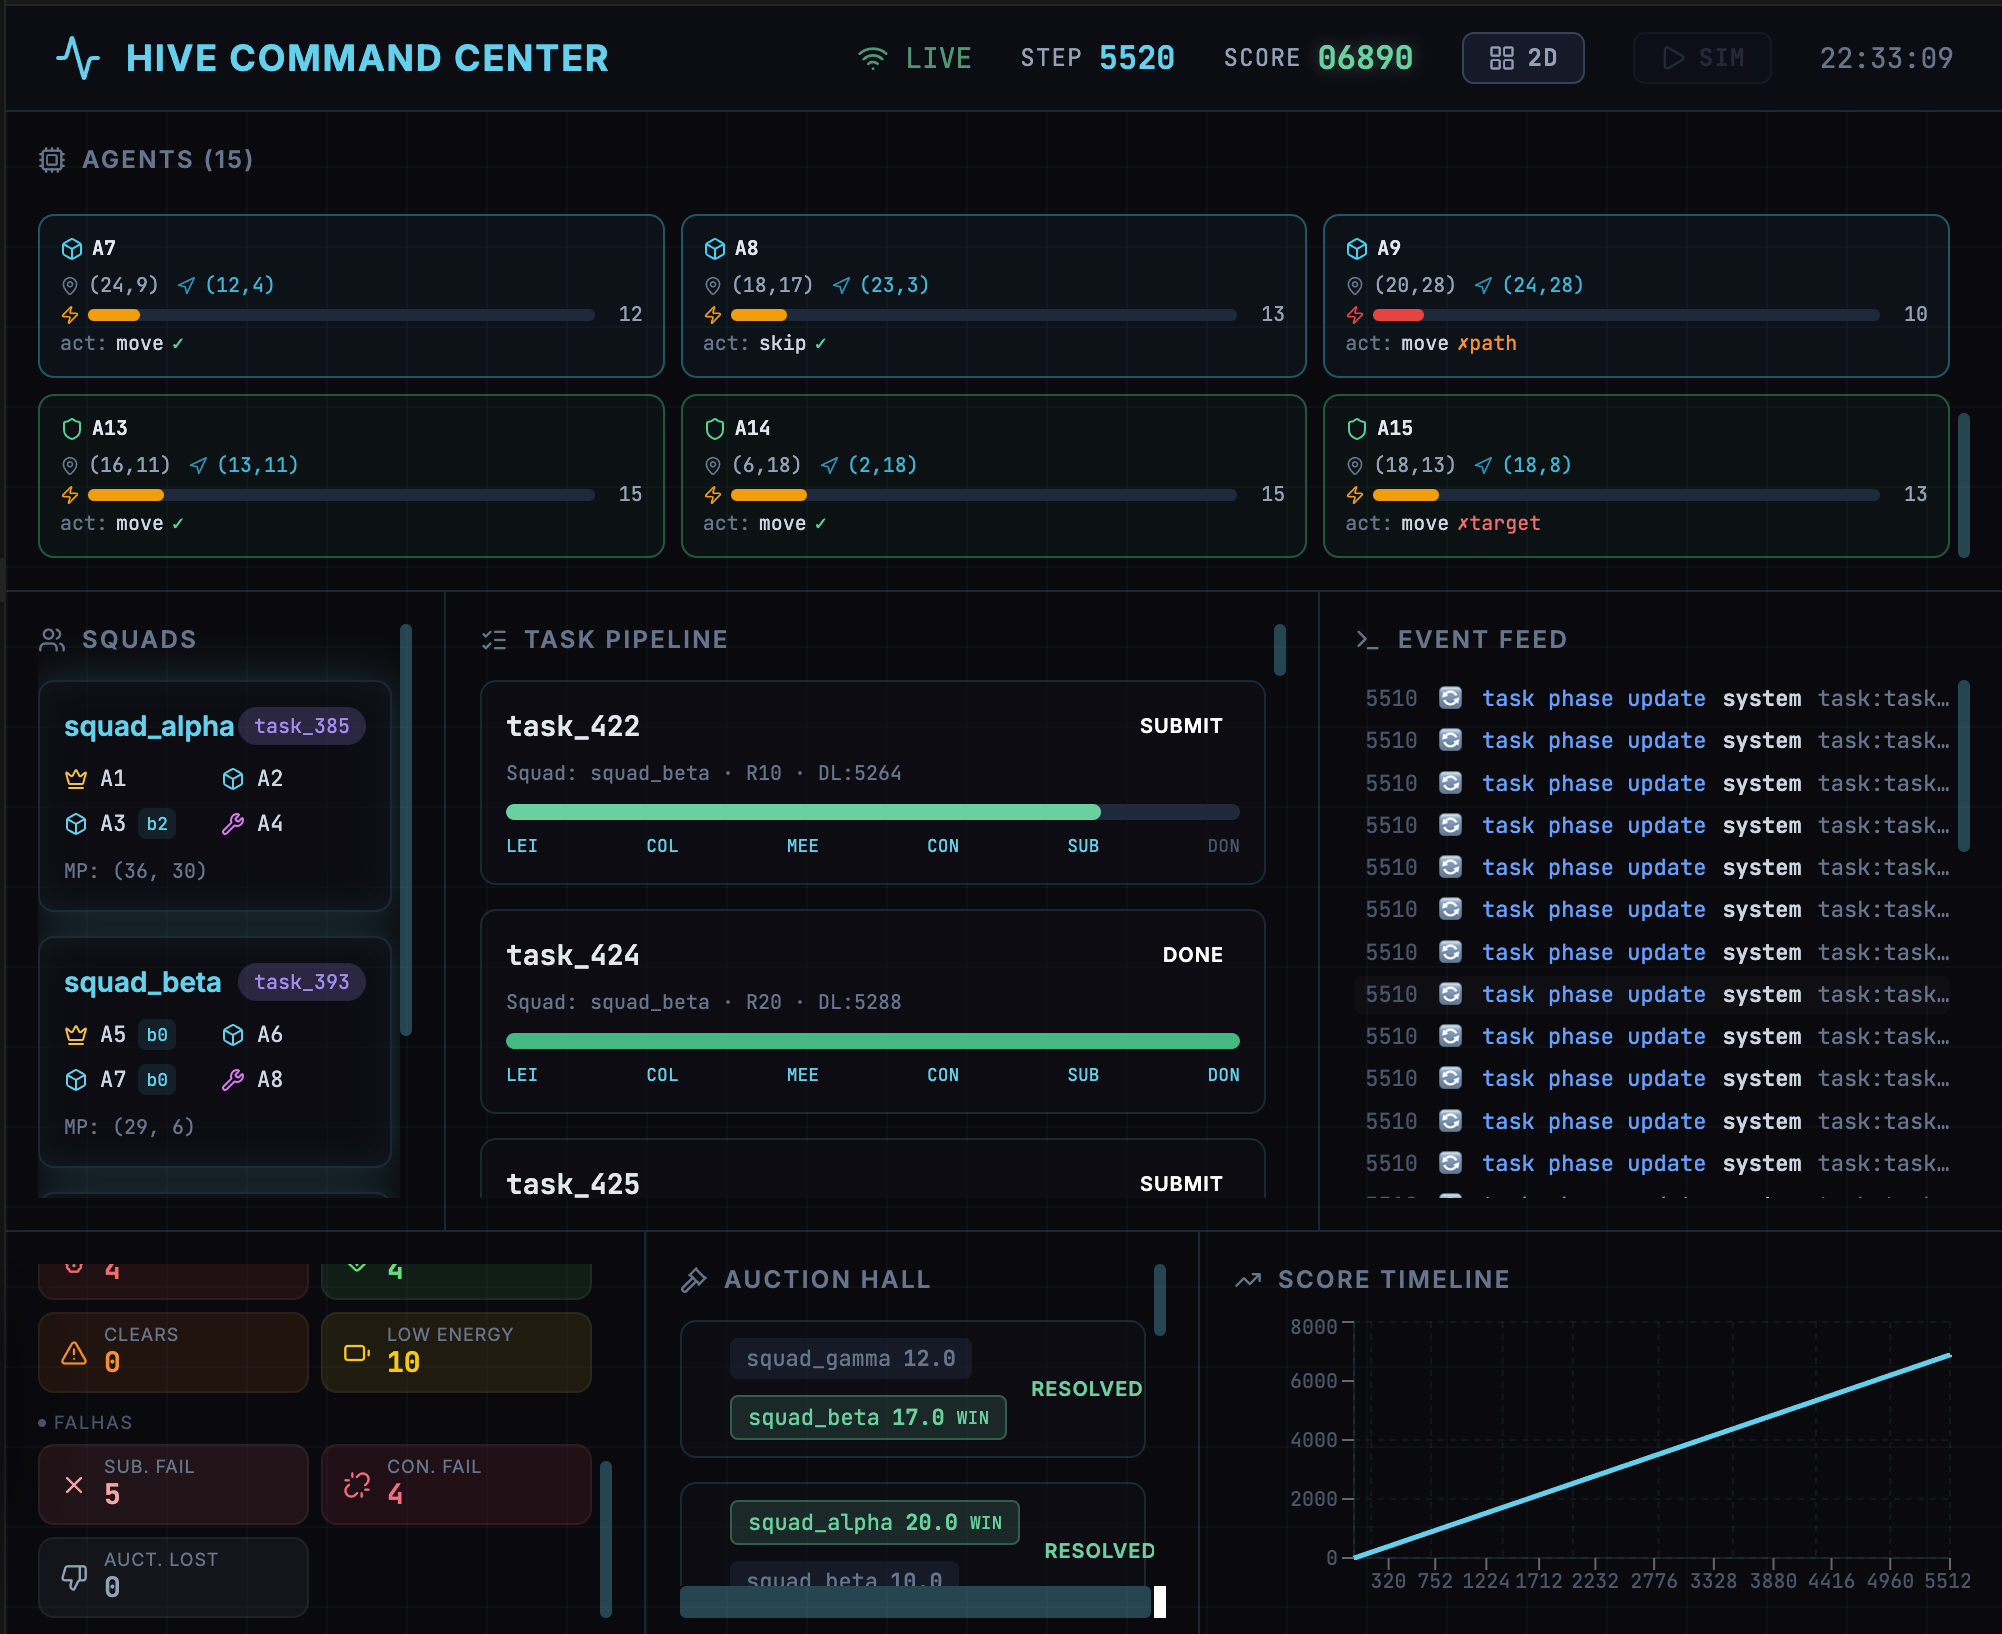
\includegraphics[width=\linewidth]{midia/hiveCommandCenter.png}
\caption{HIVE Command Center: 2D view with agents, squads, task pipeline, event feed, auction hall, battle stats, and score timeline.}
\label{fig:dash2d}
\end{figure}

\paragraph{3D View (Figure~\ref{fig:dash3d}).} The three-dimensional visualization renders the MASSim environment in an interactive perspective (orbit, pan, zoom) using React Three Fiber and Three.js:
\begin{itemize}
  \item \textbf{Agents} are cubes colored by role (yellow = leader, cyan = collector, purple = assembler, green = sentinel), with a distinct size for leaders; they move via linear interpolation, and deactivated agents fall over and become translucent;
  \item \textbf{Dispensers} appear as rotating vertical boxes colored by block type (red = b0, blue = b1, amber = b2, purple = b3);
  \item \textbf{Goal zones} are semi-transparent green planes on the grid floor;
  \item The \textbf{HUD} shows counts of agents, dispensers, and goal zones; a \textbf{legend} at the bottom identifies the visual elements.
\end{itemize}
The side panel in the 3D view keeps the Event Feed, Battle Stats, and Score Timeline visible for simultaneous monitoring.

\begin{figure}[H]
\centering
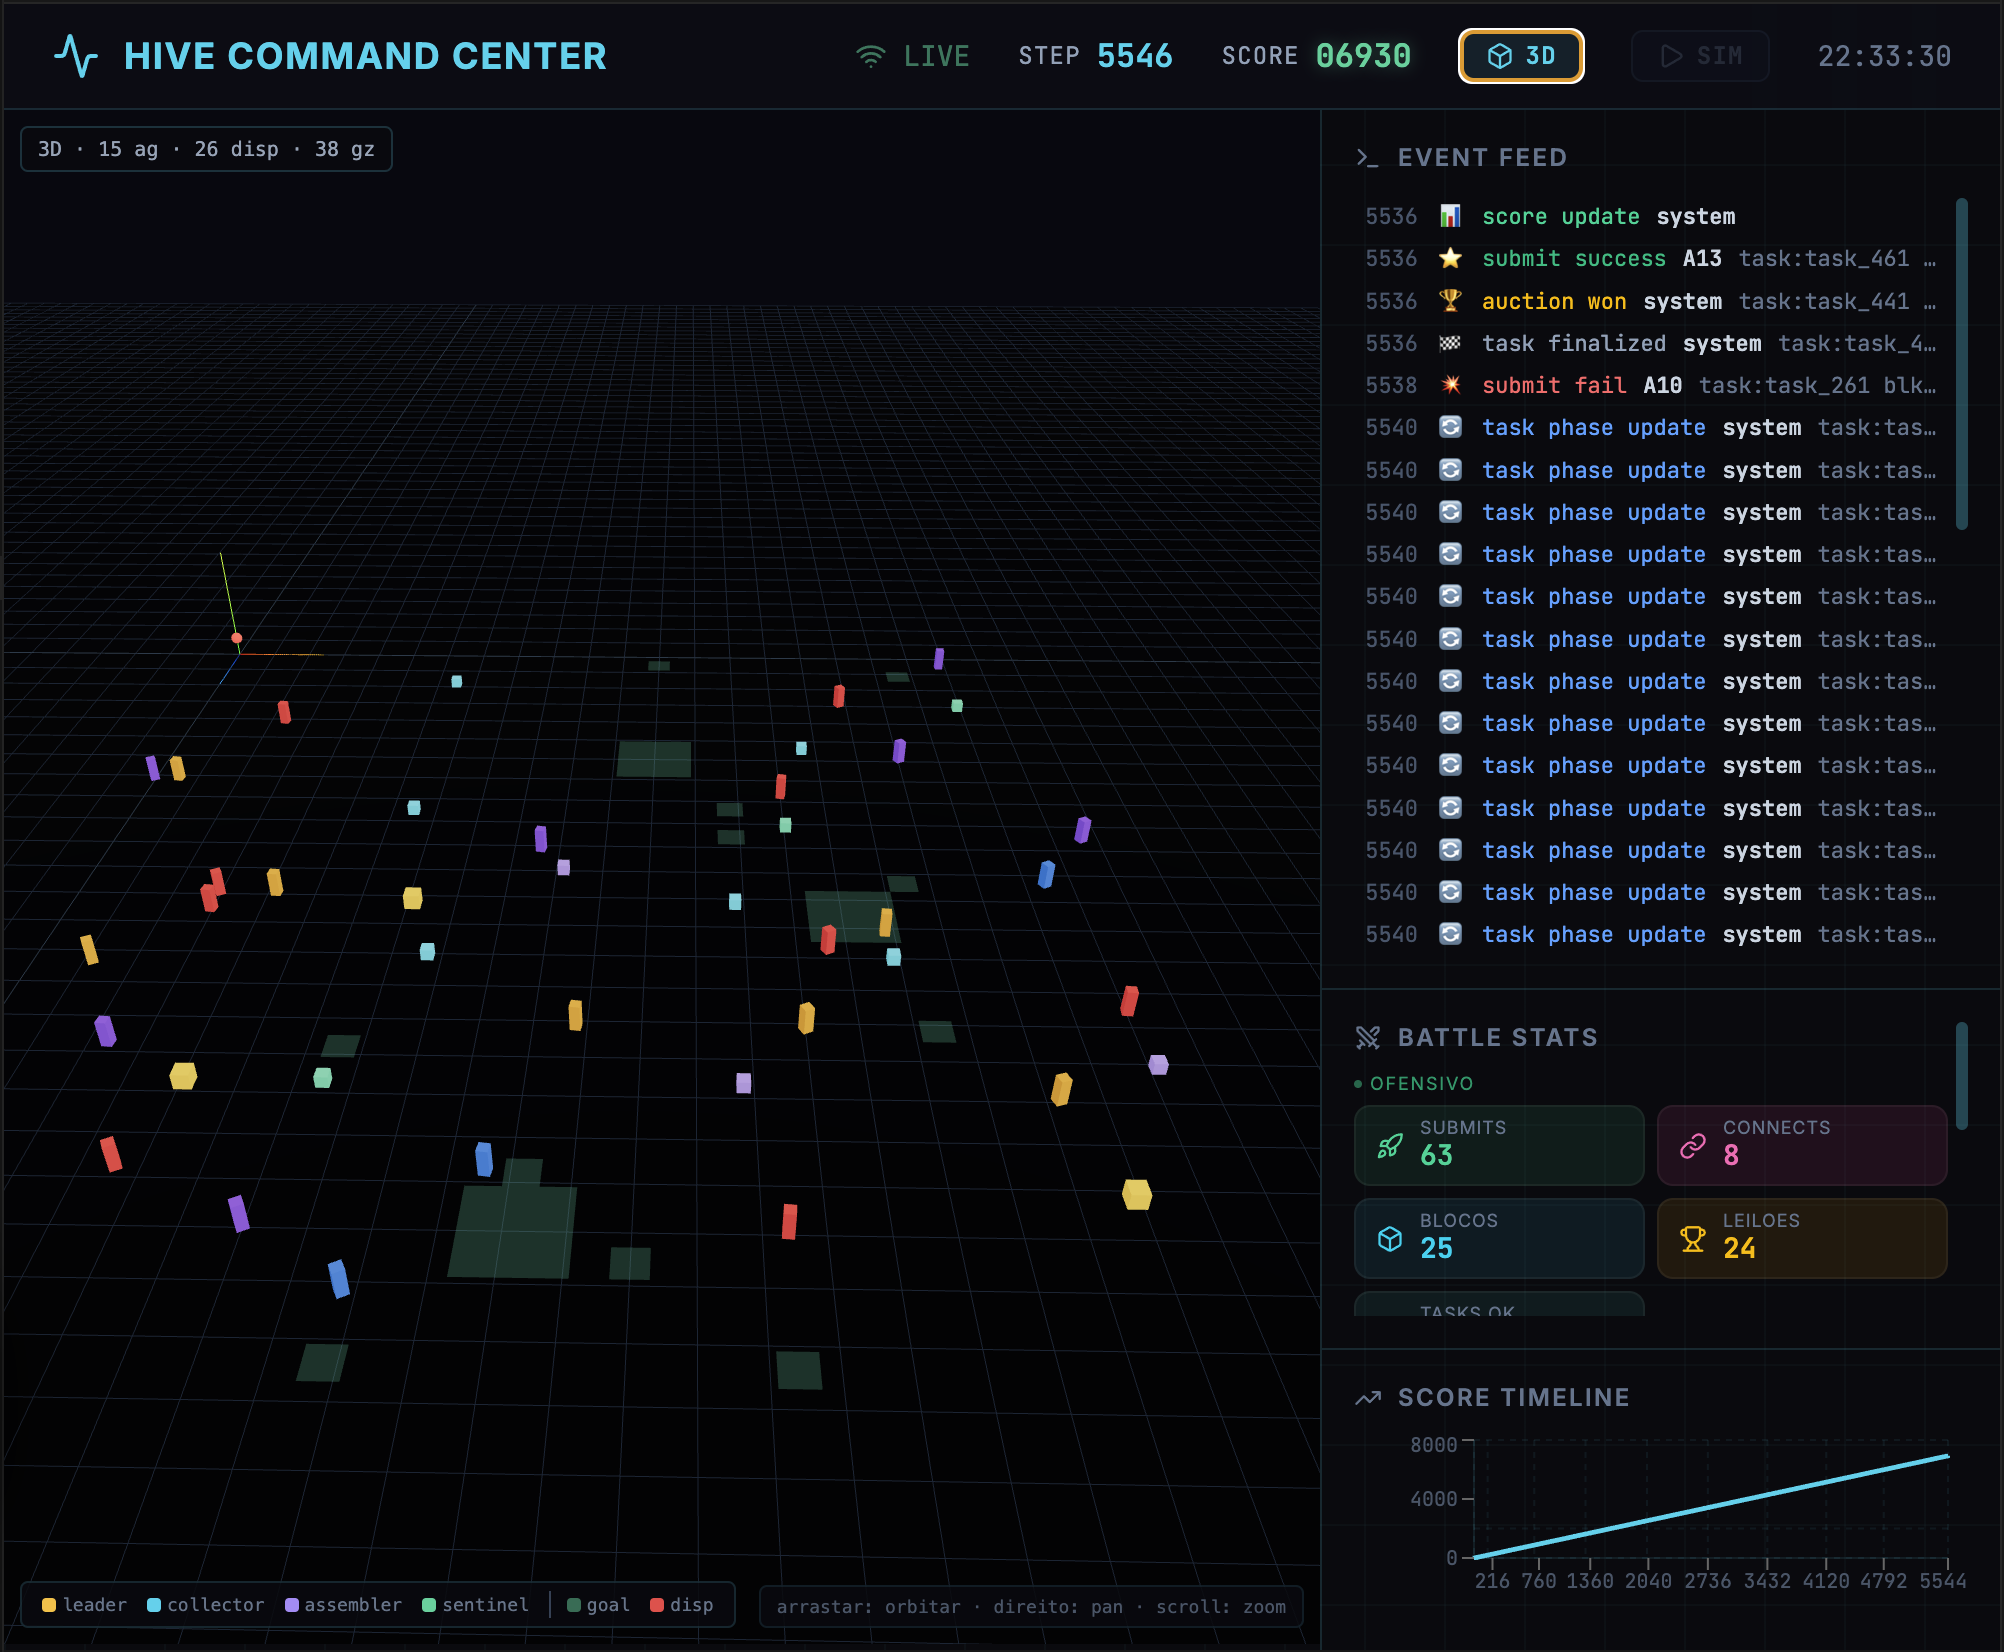
\includegraphics[width=\linewidth]{midia/hiveCommandCenter3D.png}
\caption{HIVE Command Center: 3D view with agents on the grid, rotating dispensers, goal zones, and side event panel.}
\label{fig:dash3d}
\end{figure}

The dashboard also includes an embedded \textbf{fake-simulation mode}: clicking the SIM button (when offline), the frontend internally generates simulated agents with movement, tasks, auctions, and a growing score, allowing all visual features to be demonstrated without running the MASSim server or the JaCaMo agents. When a real simulation is in progress (via WebSocket), the button is automatically disabled.

% ==============================================================
\section{Programming Languages and Execution Platform}

\subsection{JaCaMo and the MAOP Paradigm}
The \textbf{JaCaMo} platform [6, 7] implements the Multi-Agent Oriented Programming (MAOP) paradigm, which decomposes a MAS into three orthogonal dimensions:

\begin{table}[H]
\centering
\begin{tabularx}{\linewidth}{l l l X}
\toprule
\textbf{Dimension} & \textbf{Technology} & \textbf{Language} & \textbf{Central abstraction} \\
\midrule
Agent & Jason [8] & AgentSpeak(L) & Beliefs, Plans, Intentions \\
Environment & CArtAgO [11] & Java & Artifacts, Operations, Observable properties \\
Organization & MOISE+ [9] & XML & Roles, Groups, Deontic norms \\
\bottomrule
\end{tabularx}
\end{table}

\subsection{AgentSpeak(L) / Jason}
The agents are programmed in \textbf{AgentSpeak(L)} [4, 8], a declarative language based on logic programming that translates BDI concepts into concrete constructs:

\begin{table}[H]
\centering
\footnotesize
\begin{tabularx}{\linewidth}{l X X}
\toprule
\textbf{BDI Concept} & \textbf{AgentSpeak Construct} & \textbf{Example} \\
\midrule
Belief & Literal in the belief base & \code{my\_pos(10, 20)} \\
Desire / Event & Trigger event & \code{+!go\_to(X,Y)} \\
Intention & Running plan instance & \code{+!collect(B) : ... <- ...} \\
Plan & \code{event : context <- body} & \code{+!go\_to(X,Y) : my\_pos(X,Y) <- true.} \\
\bottomrule
\end{tabularx}
\end{table}

Jason's \textbf{reasoning cycle} implements the BDI loop in 10 steps [8]: perception $\rightarrow$ BRF $\rightarrow$ event generation $\rightarrow$ event selection $\rightarrow$ relevant plans $\rightarrow$ applicable plans $\rightarrow$ plan selection $\rightarrow$ intention update $\rightarrow$ intention selection $\rightarrow$ execution. This cycle is \textbf{interpreted}, granting expressiveness but introducing overhead relative to compiled implementations.

\subsection{CArtAgO}
Artifacts are implemented as \textbf{Java classes} extending \code{cartago.Artifact} [11]. Each operation is annotated with \code{@OPERATION} and may define output parameters with \code{OpFeedbackParam}. Observable properties are declared via \code{defineObsProperty} and updated with \code{updateObsProperty}, generating belief events in the agents that focus the artifact.

The \textbf{per-artifact serialization} [12] ensures that all invocations on the same artifact are processed sequentially, eliminating the need for explicit locks but limiting throughput under high concurrency.

\subsection{MOISE+}
The organizational specification is declared in \textbf{XML} following the MOISE+ model [9, 10], with three documents: structural (roles, groups, relations), functional (schemes, missions, goals), and deontic (obligations and permissions binding roles to missions). The MOISE+ runtime within JaCaMo automatically enforces norm compliance by the agents.

\subsection{Implementation Characteristics}
\begin{table}[H]
\centering
\begin{tabularx}{\linewidth}{X l}
\toprule
\textbf{Characteristic} & \textbf{Value} \\
\midrule
Lines of AgentSpeak(L) & $\sim$3{,}500 (.asl modules) \\
Lines of Java (artifacts + connection) & $\sim$2{,}500 \\
.asl files & $\sim$14 (10 common + 4 roles) \\
CArtAgO artifacts & 4 (SharedMap, TaskBoard, SquadCoordinator, HiveDashboard) \\
MOISE+ configuration & 1 XML file (\code{hive\_org.xml}) \\
Build system & Gradle + Java 21 \\
\bottomrule
\end{tabularx}
\end{table}

% ==============================================================
\section{Strategy for the Agent Team}

\subsection{Movement Algorithm}
Navigation on the 40$\times$40 toroidal grid uses two complementary algorithms:

\paragraph{A* with toroidal wrapping:} used when the toroidal Manhattan distance to the destination is $\le$ 60. The heuristic is $\min(|\Delta x|, W-|\Delta x|) + \min(|\Delta y|, H-|\Delta y|)$, which is admissible and guarantees optimality. The expansion limit is 2{,}000 nodes, falling back to greedy if exceeded. Registered obstacles expire after 30 steps to accommodate environmental changes.

\paragraph{Greedy navigation:} used for distances $>$ 60 or as an A* fallback. It computes the cardinal direction that minimizes the toroidal Manhattan distance to the destination.

\paragraph{Frontier-based exploration:} the \code{SharedMap} keeps a cache of \textbf{frontiers} (free cells adjacent to unvisited cells). Agents query \code{get\_nearest\_frontier} to select the next exploration destination, progressively covering the map.

\subsection{Coordination Strategy}
Coordination is carried out at three levels:

\paragraph{Level 1 --- Organizational (MOISE+):} the structure of 4 squads with local autonomy ensures that a leader's failure does not impact the other squads. Each leader makes allocation decisions independently.

\paragraph{Level 2 --- Distributed auction (adapted Contract Net)} [22]: the task-allocation flow follows the steps below.

\begin{enumerate}
  \item MASSim announces a new task (percept) $\rightarrow$ TaskBoard executes \code{register\_task};
  \item Leaders L1 and L2 submit \code{place\_bid(score)} to the TaskBoard;
  \item L1 invokes \code{resolve\_auction} $\rightarrow$ TaskBoard returns winner = L1;
  \item L1 calls \code{find\_free\_soloist(dispX,dispY)} on the SquadCoordinator $\rightarrow$ returns C3;
  \item L1 sends \code{.send(achieve, go\_collect(...))} to Collector C3;
  \item C3 navigates $\rightarrow$ collects $\rightarrow$ \code{submit(task)} on MASSim $\rightarrow$ +10 points.
\end{enumerate}

Two adaptations relative to the classic CNP: (i) \textbf{distributed manager} --- any leader resolves the auction, with no central point of failure; (ii) \textbf{universal contractor} --- any free agent can be a soloist, regardless of its role.

\paragraph{Level 3 --- Self-assignment:} idle agents self-assign an available task every 5 steps, without communication overhead.

\subsection{Adaptation to the Official Scenario}
The official MAPC 2022 configuration imposes three differences with strong impact on team strategy, absent from the development configuration:

\paragraph{Reactive role adoption:} in the official setting, the initial \code{default} role \textbf{does not include} the actions \code{request}, \code{attach}, \code{connect}, and \code{submit} --- the agent must be on a \emph{role zone} and execute \code{adopt(worker)} to enable them. HIVE detects this mode \textbf{reactively and self-detectably}: upon receiving the failure code \code{failed\_role} (which never occurs in dev, where \code{default} has all actions), the agent prioritizes navigation to the nearest \emph{role zone} and adopts \code{worker}. Of the five official roles (\code{default}, \code{worker}, \code{constructor}, \code{explorer}, \code{digger}), HIVE universally adopts \code{worker}, since it is the only one combining all collect-assemble-submit actions and is the fastest without load (\code{speed [2,1,1,0]}).

\paragraph{Relative positioning (dead-reckoning):} with \code{absolutePosition: false}, the agent perceives only relative coordinates. Each agent keeps a private local frame, integrating each successful move, and the shared map becomes a per-agent instance (\code{map\_<name>}). Coordinates exchanged by message are \emph{cross-frame}; map fusion requires a mutual-sighting \emph{handshake} (future work).

\paragraph{Grid dimension inference:} the official grid (70$\times$70) is larger than the development one (40$\times$40); A* operates with graceful degradation when the real toroidal dimensions are not inferred at runtime.

\subsection{Task Optimization}
The iterative optimization process led to the following critical improvements:

\begin{table}[H]
\centering
\begin{tabularx}{\linewidth}{X X}
\toprule
\textbf{Optimization} & \textbf{Impact} \\
\midrule
Reduce delegation from 3$\rightarrow$1 soloist/task & Score 20$\rightarrow$80 (+300\%) --- eliminated agent waste \\
Leader scan: 1 task per scan (every 10 steps) & Score 40$\rightarrow$100 --- eliminated timeouts from heavy loops \\
Remove \code{.wait()} from quick\_delegate & Latency reduction ($\sim$10ms per delegation) \\
Toroidal distance in \code{find\_free\_soloist} & Correct selection of the nearest soloist \\
Task timeout 200$\rightarrow$300 steps & Agents complete tasks on hard maps \\
Obstacle decay every 10 steps & 93\% reduction in decay calls \\
JVM heap 256MB$\rightarrow$2GB & Eliminated GC pauses \\
\bottomrule
\end{tabularx}
\end{table}

\subsection{Life Cycle of a Task (1 block)}
\begin{table}[H]
\centering
\begin{tabularx}{\linewidth}{l X}
\toprule
\textbf{Stage} & \textbf{Action} \\
\midrule
Step N & Server announces task T1 \\
Step N+1 & Leader: bid $\rightarrow$ auction $\rightarrow$ delegate to soloist \\
Steps N+2..k & Soloist navigates via A* to the dispenser \\
Step N+k & \code{request} + \code{attach}: block collected \\
Steps k+1..m & Navigate with the block to the goal zone \\
Step N+m & \code{submit} $\rightarrow$ +10 points \\
\bottomrule
\end{tabularx}
\caption{Life cycle of a single-block task (30--80 steps).}
\end{table}

% ==============================================================
\section{Technical Characteristics}

\subsection{Experimental Configuration}
HIVE is designed for the \textbf{official} MAPC 2022 scenario, but the systematic experimental study was conducted in a reduced \textbf{development scenario}, which enables fast iterations and isolates variables. The table contrasts the two configurations:

\begin{table}[H]
\centering
\begin{tabularx}{\linewidth}{X X X}
\toprule
\textbf{Parameter} & \textbf{Development} & \textbf{Official (competition)} \\
\midrule
Grid & 40$\times$40, toroidal & 70$\times$70, toroidal \\
Map & Cave, density 0.45 & Cave, density 0.6 \\
Steps & 800 & 750 \\
Agents (per team) & 6--20 (scale study) & 20 \\
Simultaneous teams & 1 & 2 \\
Task size & 1--2 blocks & 1--4 blocks \\
Absolute position & Enabled & \textbf{Disabled} (relative) \\
Initial role & \code{default} with all actions & \code{default} without collect/submit \\
\bottomrule
\end{tabularx}
\end{table}

The performance study below refers to the \textbf{development scenario}, in which the 15-agent configuration was identified as the best balance for the 40$\times$40 grid; the system delivered for the competition runs with 20 agents in the official scenario.

\subsection{Performance (development scenario)}
13 simulations were run with 15 agents (3L + 6C + 3A + 3S), of which 7 completed:

\begin{table}[H]
\centering
\begin{tabularx}{\linewidth}{c c c X}
\toprule
\textbf{Run} & \textbf{Score} & \textbf{Submissions} & \textbf{Status} \\
\midrule
1 & 100 & 10 & Completed \\
2 & 90 & 9 & Completed \\
3 & 80 & 8 & Completed \\
4 & 80 & 8 & Completed \\
5 & 70 & 7 & Completed \\
6 & 60 & 6 & Completed \\
7 & 60 & 6 & Completed \\
8--13 & --- & --- & Crash (steps 76--230) \\
\bottomrule
\end{tabularx}
\end{table}

\noindent\textbf{Statistics:} Mean 77.1 $\mid$ Median 80 $\mid$ Max 100 $\mid$ Min 60 $\mid$ $\sigma$ = 14.6 $\mid$ Completion rate 53.8\%.

\subsection{Scalability}
\begin{table}[H]
\centering
\begin{tabularx}{\linewidth}{c X c c}
\toprule
\textbf{Agents} & \textbf{Composition} & \textbf{Mean score} & \textbf{Crash rate} \\
\midrule
6 & 1L + 3C + 1A + 1S & 23.3 & 25\% \\
10 & 2L + 4C + 2A + 2S & 46.7 & 40\% \\
\textbf{15} & \textbf{3L + 6C + 3A + 3S} & \textbf{77.1} & \textbf{46\%} \\
20 (official) & 4L + 8C + 4A + 4S & 70.0 & 50\% \\
\bottomrule
\end{tabularx}
\end{table}

On the reduced 40$\times$40 grid, the score grows with the number of agents up to 15, stabilizing afterward. With 20 agents, the mean drops slightly in this development scenario (70 vs 77), suggesting saturation with at most 4 simultaneous tasks. It is worth noting that the official scenario (larger 70$\times$70 grid, with more dispensers and goal zones) mandates 20 agents --- a configuration in which the saturation observed on the small grid does not apply in the same way.

\subsection{Stability and Failure Diagnosis}
About \textbf{46\% of the runs} do not complete the 800 steps. Log analysis revealed a consistent pattern:
\begin{enumerate}
  \item \textbf{Trigger} (steps 76--230): 15 agents process percepts simultaneously, generating $\sim$600--900 \code{mark\_obstacle} calls per step --- all serialized in the \code{SharedMap} artifact [12];
  \item \textbf{Escalation}: the serialized time exceeds the 8-second timeout;
  \item \textbf{Collapse}: the EIS library interprets the timeout as a connection failure and starts a flood of reconnections;
  \item \textbf{Terminal loop}: the disconnect/reconnect cycle becomes self-sustaining indefinitely.
\end{enumerate}

The collapse pattern is a causal chain: \emph{15 agents process percepts} ($\sim$900 \code{mark\_obstacle}/step) $\rightarrow$ \emph{CArtAgO serialization $>$ 8s} $\rightarrow$ \emph{server logs ``No valid action''} $\rightarrow$ \emph{EIS attempts to reconnect} $\rightarrow$ \emph{flood of reconnections}, which feeds back into the reconnection attempt, sustaining the loop indefinitely.

\noindent\textbf{Evidence:} reducing the cave density from 0.45 to 0.25 dropped the crash rate to \textbf{0\%}, confirming that the volume of obstacle percepts is the determining factor. This limitation is inherent to the CArtAgO serialization model [12] --- it is not a defect in the agents' logic.

\subsection{Failure Recovery}
HIVE implements recovery mechanisms in the following scenarios:
\begin{itemize}
  \item \textbf{Stuck agent} (\emph{stuck detection}): if an agent stays in the same position for 50 steps, the \code{need\_detach} mechanism is triggered --- the agent detaches blocks and looks for an alternative route;
  \item \textbf{Goal-zone blockage}: if an agent with \code{pending\_submit} is blocked for 6+ movement attempts, it seeks an alternative goal zone via \code{get\_alternative\_goal\_zone};
  \item \textbf{Task expiration}: tasks pending for more than 300 steps are abandoned and the agent returns to the soloist pool;
  \item \textbf{Obstacle expiration}: obstacles in the \code{SharedMap} expire after 30 steps, avoiding permanently invalid routes;
  \item \textbf{EIS timeout}: the EIS client was configured with an 8{,}000ms timeout, aligned with the server, to avoid premature disconnections.
\end{itemize}

\subsection{Comparison with MAPC 2022}
\begin{table}[H]
\centering
\begin{tabularx}{\linewidth}{c X l c}
\toprule
\textbf{Position} & \textbf{Team} & \textbf{Framework} & \textbf{Typical score} \\
\midrule
1st & FIT-BUT [17] & Pure Java & 200--400 \\
2nd & MMD [18] & Java (optimization) & 150--300 \\
--- & LI(A)RA [19] & JaCaMo & 80--150 \\
--- & \textbf{HIVE} & \textbf{JaCaMo} & \textbf{60--100} \\
\bottomrule
\end{tabularx}
\end{table}

The gap to the top teams is attributed to the \textbf{low completion rate of multi-block tasks}: the single-block pipeline works reliably, but the \emph{connect} protocol rarely completes successfully on dense cave maps. Teams such as FIT-BUT [17] use pure Java with direct thread control, avoiding CArtAgO's serialization bottleneck.

% ==============================================================
\section{Discussion and Conclusion}

\subsection{Ease/Difficulty of the MAOP Method}
The MAOP approach via JaCaMo [6] demonstrated \textbf{high conceptual expressiveness}: the separation into agents/environment/organization mapped directly onto the theoretical MAS concepts studied in the PCS 5703 course [1]. Programming in AgentSpeak(L) [8] allowed complex behaviors to be expressed declaratively and modularly.

However, Jason's \textbf{interpreted} nature --- unifying plans against the belief base every step --- introduces significant overhead under high load: with 15--20 agents each running hundreds of beliefs, deliberation time becomes a limiting factor. This observation is consistent with the LTI-USP experience [20] in earlier MAPC editions.

The trade-off between \textbf{declarative expressiveness} and \textbf{computational efficiency} is the main tension found: interpreted BDI frameworks offer traceability and conceptual fidelity but lose performance to compiled Java implementations [17].

\subsection{Ease/Difficulty of the Organizational Model}
MOISE+ [9, 10] provided a clear and verifiable organizational structure that facilitated the system's top-down design. The division into 4 squads with local autonomy demonstrated the concept of \textbf{decentralized organization}.

However, MOISE+ is primarily \textbf{declarative and static}: it defines \emph{who can do what}, but not \emph{when} or \emph{how} coordination occurs at runtime. Dynamic coordination --- deciding which agent takes which task, when to abandon a task --- was implemented entirely in AgentSpeak plans and CArtAgO artifacts, not in the organizational model. For highly dynamic scenarios like the MAPC, MOISE+ works better as a \textbf{structural framework} than as an \textbf{operational coordination mechanism}.

\subsection{CArtAgO: Power and Limitations}
CArtAgO artifacts [11, 13] validated the central premise of the A\&A meta-model [13] --- artifacts as tools that mediate collective activity. The \code{SharedMap} encapsulated A*, exploration, and obstacles in a clean interface; the \code{TaskBoard} implemented the auction without the agents knowing the protocol.

However, the \textbf{per-artifact serialization} [12] proved to be the main bottleneck. One solution would be \textbf{functional partitioning} (sharding): splitting the \code{SharedMap} into smaller per-function artifacts (obstacles, dispensers, goal zones), distributing the serialization load.

\subsection{Adaptation to the Official Scenario}
Migrating from the development configuration to the official scenario exposed valuable lessons. The initial \code{default} role enables neither collection nor submission: the agent must adopt \code{worker} on a \emph{role zone}. The \textbf{reactive} implementation of this mechanism --- triggered by the \code{failed\_role} failure code, without static mode flags --- proved consistent with the BDI principle of perception-guided adaptation [3, 8] and avoided rigid assumptions about the environment. The \textbf{relative positioning} (\code{absolutePosition: false}), handled by dead-reckoning with a per-agent local frame, revealed the cost of giving up a global reference: map fusion among agents (a prerequisite for reliable multi-block rendezvous) requires a mutual-sighting \emph{handshake}, left as future work. These adaptations confirm that seemingly small scenario decisions (per-role actions, coordinate reference frame) have deep architectural impact.

\subsection{Possible Extensions}
\begin{enumerate}
  \item \textbf{Artifact sharding}: partition the \code{SharedMap} to reduce serialization contention;
  \item \textbf{Robust multi-block pipeline}: redesign the \emph{connect} protocol with dynamic meeting points and fault tolerance;
  \item \textbf{Map fusion in relative mode}: mutual-sighting \emph{handshake} to translate dead-reckoned frames into a common reference;
  \item \textbf{Self-assignment with spatial affinity}: lightweight dispersion based on position hashing, without \code{findall};
  \item \textbf{Asynchronous CArtAgO operations}: non-blocking operations for map updates;
  \item \textbf{Reinforcement learning for parameters}: automatic tuning of thresholds and frequencies.
\end{enumerate}

\subsection{Conclusion}
This work presented HIVE, a JaCaMo-based MAS [6] for the Agents Assemble scenario of MAPC 2022 [14]. The system demonstrates the integrated application of the three MAOP pillars: BDI agents in Jason [8], normative organization in MOISE+ [9], and shared environment in CArtAgO [11].

The experimental results --- scores of 60--100 points with a mean of 77 in the development scenario --- validate the feasibility of the MAOP paradigm [7] for complex multi-agent coordination scenarios, while the scalability analysis (15 agents as the best balance on the reduced grid; 20 agents in the official configuration) and the instability diagnosis (CArtAgO serialization bottleneck) contribute practical insights to the community.

The main contribution goes beyond the numerical results: the experience concretely exposed the trade-offs theorized in the literature --- between autonomy and coordination [1], between expressiveness and efficiency [8], between consistency and concurrency [12]. As argued by Bratman [3], rational agents need intentions as commitments that reduce the deliberation space. HIVE shows that this need applies to the \textbf{system as a whole}: the choice of framework, the granularity of artifacts, and the coordination frequency are themselves design commitments that determine the MAS's success in competitive and dynamic environments.

% ==============================================================
\section*{References}
\addcontentsline{toc}{section}{References}
{\small
\begin{list}{}{\setlength{\leftmargin}{2.0em}\setlength{\itemindent}{-2.0em}\setlength{\itemsep}{3pt}}

\item [1] M. Wooldridge, \emph{An Introduction to MultiAgent Systems}, 2nd ed. Chichester, UK: John Wiley \& Sons, 2009.
\item [2] M. Wooldridge and N. R. Jennings, ``Intelligent agents: Theory and practice,'' \emph{The Knowledge Engineering Review}, vol. 10, no. 2, pp. 115--152, 1995.
\item [3] M. E. Bratman, \emph{Intention, Plans, and Practical Reason}. Cambridge, MA: Harvard University Press, 1987.
\item [4] A. S. Rao and M. P. Georgeff, ``BDI Agents: From Theory to Practice,'' in \emph{Proc. 1st Int. Conf. on Multiagent Systems (ICMAS-95)}, 1995, pp. 312--319.
\item [5] A. S. Rao and M. P. Georgeff, ``Modeling Rational Agents within a BDI-Architecture,'' in \emph{Proc. 2nd Int. Conf. on Principles of Knowledge Representation and Reasoning (KR'91)}, 1991, pp. 473--484.
\item [6] O. Boissier, R. H. Bordini, J. F. Hübner, and A. Ricci, \emph{Multi-Agent Oriented Programming: Programming Multi-Agent Systems Using JaCaMo}. Cambridge, MA: MIT Press, 2020.
\item [7] O. Boissier, R. H. Bordini, J. F. Hübner, A. Ricci, and A. Santi, ``Multi-agent oriented programming with JaCaMo,'' \emph{Science of Computer Programming}, vol. 78, no. 6, pp. 747--761, 2013.
\item [8] R. H. Bordini, J. F. Hübner, and M. Wooldridge, \emph{Programming Multi-Agent Systems in AgentSpeak using Jason}. Chichester, UK: John Wiley \& Sons, 2007.
\item [9] J. F. Hübner, J. S. Sichman, and O. Boissier, ``Developing organised multiagent systems using the MOISE+ model,'' \emph{Int. J. of Agent-Oriented Software Engineering}, vol. 1, no. 3/4, pp. 370--395, 2007.
\item [10] J. F. Hübner, J. S. Sichman, and O. Boissier, ``A Model for the Structural, Functional and Deontic Specification of Organizations in Multiagent Systems,'' in \emph{SBIA 2002}, LNAI, vol. 2507. Springer, 2002, pp. 118--128.
\item [11] A. Ricci, M. Piunti, M. Viroli, and A. Omicini, ``Environment Programming in CArtAgO,'' in \emph{Multi-Agent Programming}, Springer, 2009, pp. 259--288.
\item [12] A. Ricci, M. Piunti, and M. Viroli, ``Environment programming in multi-agent systems: An artifact-based perspective,'' \emph{Autonomous Agents and Multi-Agent Systems}, vol. 23, pp. 158--192, 2011.
\item [13] A. Omicini, A. Ricci, and M. Viroli, ``Artifacts in the A\&A meta-model for multi-agent systems,'' \emph{Autonomous Agents and Multi-Agent Systems}, vol. 17, no. 3, pp. 432--456, 2008.
\item [14] T. Ahlbrecht, J. Dix, N. Fiekas, and T. Krausburg, Eds., \emph{The Multi-Agent Programming Contest 2022}, LNCS, vol. 13997. Springer, 2023.
\item [15] T. Ahlbrecht, J. Dix, N. Fiekas, and T. Krausburg, Eds., \emph{The Multi-Agent Programming Contest 2021}, LNCS, vol. 12947. Springer, 2021.
\item [16] T. Ahlbrecht, J. Dix, N. Fiekas, and T. Krausburg, ``The Multi-Agent Programming Contest: A Résumé,'' \emph{Annals of Mathematics and Artificial Intelligence}, 2020.
\item [17] F. Zboril Jr., F. Vidensky, L. Dokoupil, and J. Beran, ``FIT-BUT at MAPC 2022,'' in \emph{LNCS}, vol. 13997. Springer, 2023, pp. 120--150.
\item [18] P. Böhm, ``Optimization-Based Agents in the 16th Multi-agent Programming Contest,'' in \emph{LNCS}, vol. 13997. Springer, 2023, pp. 19--53.
\item [19] M. Custódio, M. Rocha, R. Battaglin, G. P. Farias, and A. R. Panisson, ``LI(A)RA Team --- MAPC 2022,'' in \emph{LNCS}, vol. 13997. Springer, 2023, pp. 165--194.
\item [20] M. F. Stabile Jr. and J. S. Sichman, ``The LTI-USP Strategy to the 2020/2021 Multi-Agent Programming Contest,'' in \emph{LNCS}, vol. 12947. Springer, 2021, pp. 108--133.
\item [21] M. R. Franco, L. M. Rosset, and J. S. Sichman, ``Improving the LTI-USP Team: A New JaCaMo Based MAS for the MAPC 2013,'' in \emph{EMAS 2013}, LNAI, vol. 8245. Springer, 2013, pp. 339--348.
\item [22] R. G. Smith, ``The Contract Net Protocol: High-Level Communication and Control in a Distributed Problem Solver,'' \emph{IEEE Trans. on Computers}, vol. C-29, no. 12, pp. 1104--1113, 1980.
\item [23] Multi-Agent Programming Contest, ``Scenario Description: Agents Assemble 2022.'' [Online]. \url{https://github.com/agentcontest/massim_2022/blob/main/docs/scenario.md}
\item [24] Multi-Agent Programming Contest. [Online]. \url{https://multiagentcontest.org/}
\item [25] JaCaMo Project. [Online]. \url{https://jacamo-lang.github.io/}

\end{list}
}

\end{document}
